\documentclass[conference]{IEEEtran}
\usepackage{enumitem}
\usepackage[document]{ragged2e}
\usepackage{blindtext}
\usepackage{graphicx}
\usepackage{float}
%\usepackage{natbib}
\usepackage{cite}

\graphicspath{ {./}{./images/} }

\title{Joint Radar Communication System using OFDM}

\author{

\IEEEauthorblockN{Owen Sowatzke}
\IEEEauthorblockA{\textit{Electrical Engineering Department} \\
\textit{University of Arizona}\\
Tucson, USA \\
osowatzke@arizona.edu}

\and
\IEEEauthorblockN{Iman Miraki}
\IEEEauthorblockA{\textit{Electrical Engineering Department} \\
\textit{University of Arizona}\\
Tucson, USA \\
imanmiraki@arizona.edu}}

\begin{document}
	\maketitle
\setlength{\hsize}{0.9\hsize}% emphasize effects
\RaggedRight
\section {Introduction}
     Vehicle-to-Vehicle networks seek to enhance road safety and reduce traffic congestion by sharing information between vehicles. Such networks possess enormous potential in improving driving safety and traffic conditions by sharing road and traffic information among vehicles in real-time.These systems need dedicated bandwidth to avoid delays associated with third party networks. Sharing bandwidth between existing vehicle radar and planned communication network would reduce total bandwidth usage and power consumption.\par
     The Idea behind JRC is to integrate radar sensing and wireless communication systems into a single framework, allowing vehicles to perform both tasks using the same hardware, spectrum, and waveform resources. This integration is critical for improving situational awareness, safety, and efficient use of spectrum in V2V networks.\par
     In this paper, we design a joint-radar communication (JRC) system, which uses OFDM for communication and zero-forcing to generate a range response from the OFDM returns. To evaluate the system performance, we provide the simulation results and compare Radar and Communication with JRC.
     

	\begin{enumerate}
	  \item Radar
        	  \item OFDM
         	 \item JRC\par
        
  \section {Radar}
   \subsection {Background}
   
In this section we glance through FMCW radar (Frequency-modulated Continous Wave) to familiarize ourself with the functionality, key features, and advantages of this radar topology. FMCW continuously transmits a signal whose frequency varies over time. The core principle of FMCW radar is that it measures the time delay between the transmitted signal and the reflected signal (echo) to determine the distance to an object, and the frequency shift caused by the Doppler effect is used to measure relative velocity.


Key features of FMCW are:
	\begin{itemize}
		\item Continous wave tramsmission
		\item Frequency modulation
		\item Range measurement
		\item Doppler shift
	\end {itemize}
	

 The block diagram provided below represents the signal processing chain of a typical FMCW radar system. The transmitter portion generates a chirp signal (frequency-modulated) and transmit through the antenna toward the target. Receiver path receives the reflected signal from the target, amplifies the signal, mix the signal with the transmitted signal and pass it to ADC. The signal processing portion determin the range and doppler by performing a FFT.

	\begin{figure}[H]
    		\centering
    		\fbox{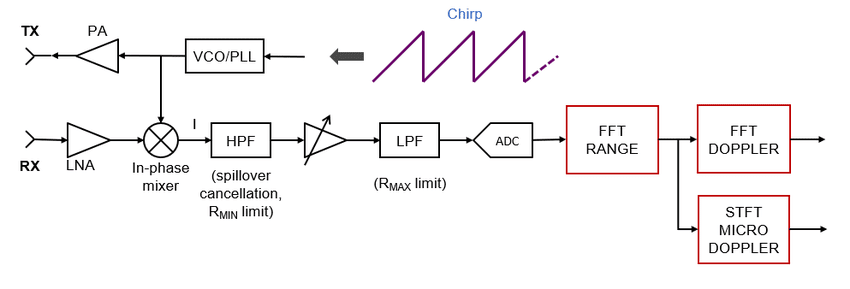
\includegraphics[width=0.9\linewidth]{FMCW Blockdiagram}}
    		\caption{Typical FMCW blockdiagram \cite{9613183}}
	\end{figure}
	
The main purpos of the radar, estimating velocity and range of the target, is acuratly achievable with FMCW signlas. The mathotalegy can be simply comprehented by the graph below. The range FFT provides the beat frequency to calculate the target distance and doppler FFT provides the frequncy delta between trnasmitted and received signal to calculate the target velocity. 
	
	\begin{figure}[H]
    		\centering
    		\fbox{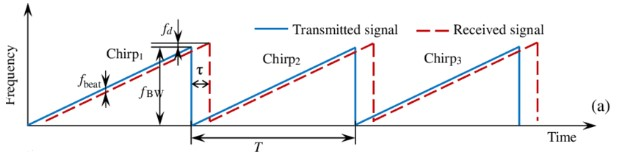
\includegraphics[width=0.8\linewidth]{FMCW Freq-Time graph}}
    		\caption{Typical FMCW transmitted and Received signal, Time vs Frequency graph \cite{Long2019AssistingTV}}
	\end{figure}
	
	Range (targer distance) can be calculated from simple formula below:
	
	\begin{figure}[H]
    		\centering
    		\fbox{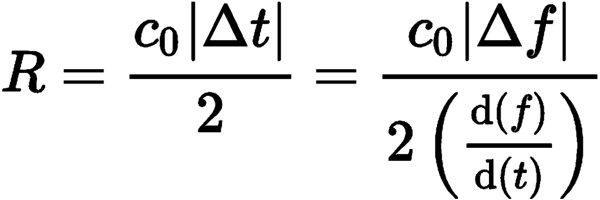
\includegraphics[width=0.5\linewidth]{Range formula}}
    		\caption{Range calculation}
	\end{figure}
	
	\begin{itemize}
	\item Co = speed of light = 3·108 m/s
	\item \(\Delta \)t = delay time [s]
	\item \(\Delta \)f = measured frequency difference [Hz]
	\item R = distance between antenna and the reflecting object (ground) [m]
	\item df/dt = frequency shift per unit of time
	\end{itemize}

In the interest of comparing FMCW with JRC methode, we outline few advantages of FMCW in radar.
	\begin{itemize}
		\item High range resolution
		\item Continuous operation
		\item Simultaneous range and velocity measurement
		\item Simple hardware
		\item Low power consumption
	\end{itemize}
	
\subsection {Simulation and Performance}

In this section we provide the results of the FMCW radar simulation that coded with Matlab. The code written programaticaly to allow us easily change the parameters to match the JRC wave and channel properties. This is necessery to have the comprehensive and fair comparison between FMCW and JRC performance. 
The results below are extracted from the FMCW  radar simulation with parameter below:
	\begin{itemize}
	\item Carrier Frequency:	77 GHz
	\item Sampling Rate:		200 MHz
	\item PRF:				500 KHz
	\item Code Length:		127
	\item SNR:				20 dB
	\end{itemize}
	
Simulation contains of generating the chirp signal for transmission, simulatin gthe received signal with target delays, Doppler shifts and noise. Windowin gis applied in both steps to reduce spectral leakage. The produced results are  FFT oerations in both fast and slow time. It supports multiple targets and includes configurable parameters like bandwidth, sample rate, and windowing functions. Graph below is the result of fast-time FFT displaying the target range.

	\begin{figure}[H]
	    		\centering
	    		\fbox{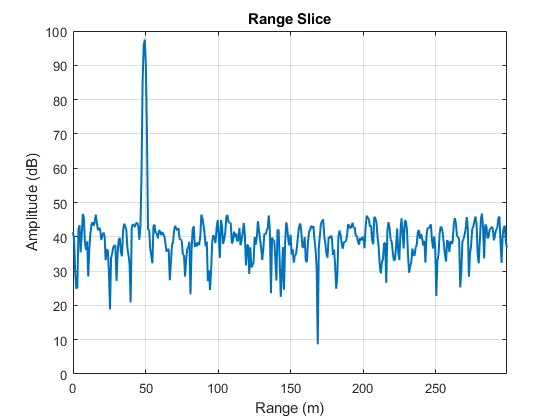
\includegraphics[width=0.8\linewidth]{FMCW_Range Slice}}
	    		\caption{FMCW range slice}
		\end{figure}

Graph below is the result of slow-time FFT, displaying the target velocity by analizing the phase change over multiple chirps. 

	\begin{figure}[H]
	    		\centering
	    		\fbox{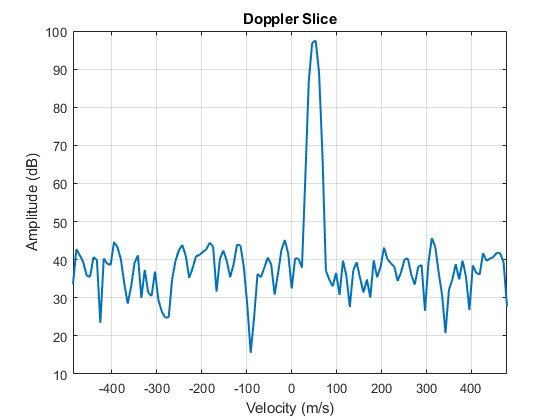
\includegraphics[width=0.8\linewidth]{FMCW_Doppler Slice}}
	    		\caption{FMCW Doppler slice}
		\end{figure}
	
Graph below is the result of mixing both Range and Doppler FFT. The Range-Doppler map's X-axis is a Doppler bins (relative velocity) and Y-axis is a range bins (distance). Bright spots indicate targets and their corresponding tange and velocity.
	\begin{figure}[H]
	    		\centering
	    		\fbox{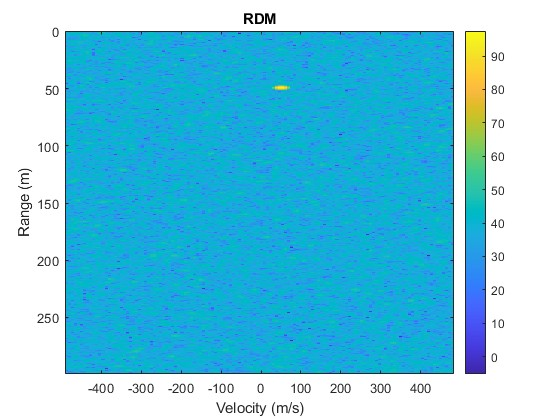
\includegraphics[width=0.8\linewidth]{FMCW_RDM}}
	    		\caption{FMCW Range Doppler Map}
		\end{figure}
		
		
     \section {Communication (OFDM)}
     
	 \subsection {Background}
 
 
            In this section we skim through OFDM communicaiton protocol. Since the objective of this paper is V2V JRC our focus is on IEEE 802.11 P standard. In this section we familiarize ourself with the functionality, key features, some 802.11 P standard specificaitons and advantages of this communication topology.\par
    \textbf{  802.11 P} is specifically designed for wireless access in vehicular environments (WAVE) and is widely used for V2V applications within the automotive industry.
      
      \begin{itemize}
      \item Frequency Band:		5.850 GHz to 5.925 GHz (DSRC Band)
	\item Channel Bandwidth:	10 MHz
	\item Modulation:		BPSK, QPSK, 16-QAM
	\item Maximum Data Rate:	27 Mbps (Theoretical)
	\item Range: 			Up to 1 km (ideal conditions)
	\item Vehicle Speed :                Up to 200 km/h
	\item Security:			WPA2, Authentication, Message Integrity
	\item Applications:		Collision avoidance, traffic management, V2X
	\end{itemize}
	
 \textbf{ Orthogonal Frequency Division Multiplexing (OFDM)} is widely used in Vehicle-to-Vehicle (V2V) communication systems for several reasons, including inherent characteristics that provide efficient data transmission in dynamic, high-speed environments.

Block diagram below is a typical OFDM process from input bit steam, modulation, through the channel, DFT, demodulation and output bit steam. 

		\begin{figure}[H]
	    		\centering
	    		\fbox{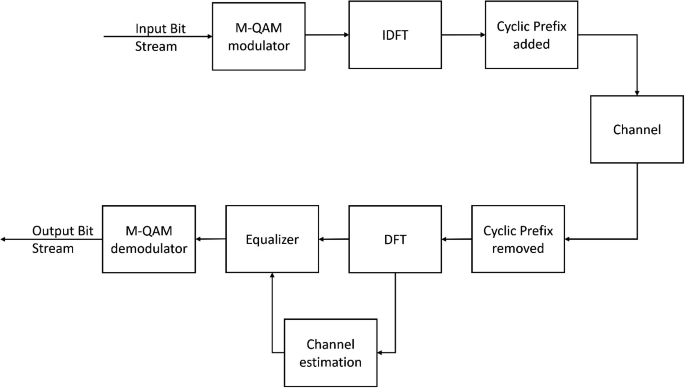
\includegraphics[width=0.9\linewidth]{OFDM Block diagram}}
	    		\caption{OFDM block diagram}
		\end{figure}
      
      The graph below illustrat a typical OFDM fram (64-subcarrier example)
      
      	\begin{itemize}
      	\item Guard Band (Zero Subcarriers): Subcarriers 0–5 and 59–63
	\item Data Subcarriers: Subcarriers 6–28 and 37–58
	\item Pilot Subcarriers: Subcarriers 7, 21, 43, 57
	\item DC Subcarrier (Zero): Subcarrier 32
	\end{itemize}

	\begin{figure}[H]
	    		\centering
	    		\fbox{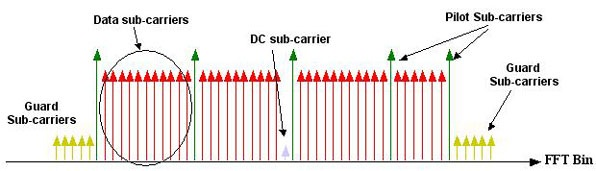
\includegraphics[width=0.9\linewidth]{OFDM subcarriers}}
	    		\caption{OFDM subcarriers}
		\end{figure}
		
One othere channels' property needs to be analysed and compared is the channel capacity. We use the simple fromula below to calculate the channel capacity. 
Where H (m, n) , Hmn is the channel frequency response of the n symbol on the m sub carrier. 
	
	\begin{figure}[H]
	    		\centering
	    		\fbox{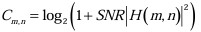
\includegraphics[width=0.9\linewidth]{Capacity Formula}}
	    		\caption{OFDM Capacity calculation}
		\end{figure}

\subsection {Simulation and Performance}
      
      We have developed comprehensive MATLAB code to evaluate and plot the Bit Error Rate (BER) versus SNR across various channel conditions.. Evaluating diverse channel characteristics is key to achieving a comprehensive and unbiased analysis in our study. The summary implemntation of a complete OFDM simulation model parameters and results for AWGN, Rayleight Fading and perfect channel provided below. 
      
\begin{itemize}
\item 64 Subcarriers, 48 Data carriers, 10 K Symbols adn 16 Cyclic-prefix
\item 4th order QAM modulation and 10 MHz Sample rate
\item Pilots are inserted at standard intervals and zero carriers are placed at the edges of the spectrum.
\item The IFFT converts the frequency domain symbols to the time domain. 
\item A Hamming window is applied to each OFDM symbol to reduce spectral leakage. 
\item A cyclic prefix is added to the windowed OFDM symbols to mitigate ISI. 
\item An AWGN channel is used to transmit the flattened signal to the receiver.\par
\item The receiver removes the cyclic prefix. 
\item The data sub-carriers are extracted and demodulated from FFT, results in frequency domain. 
\item The received bits are compared to the transmitted bits to calculate the BER vs SNR values. 
\end{itemize}
The power spectral density of trasmitted OfDM signal shown in the graph below. The flat region conrresponds to the active subcarriers of the OFDM signal (each subcarrier carries equal power and spans the same bandwidth). There is a dip null in the center correspoinding to the DC (zero frequency) subcarrier which used to avoid interference. The dips at the edges are the guard bands to rduce spectral leakage and interference with adjacent channels.

	\begin{figure}[H]
    		\centering
    		\fbox{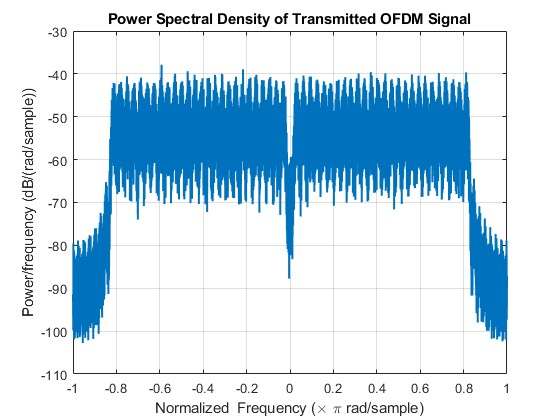
\includegraphics[width=0.8\linewidth]{OFDM Power spectral density}}
    		\caption{OFDM Power Spectral Density}
	\end{figure}

  The graph below is a constellation coresponding to 4th order QAM with AWGN channel propery.  The points are tightly packed around the ideal constellation locations, indicating that noise has minimal impact on the received signal (high SNR conditions).This diagram demonstrates that the system performs well under high SNR conditions, maintaining accurate symbol transmission and reception.
    
    
     \begin{figure}[H]
		\centering
    		\fbox{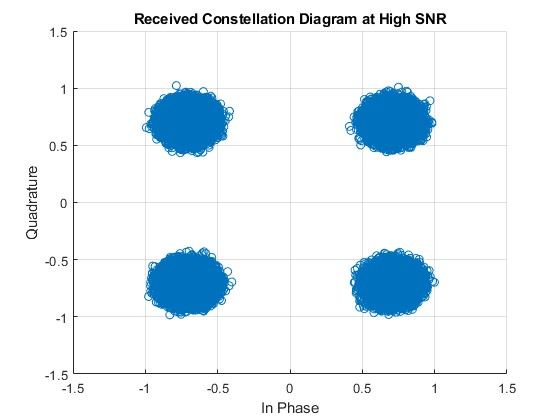
\includegraphics[width=0.8\linewidth]{OFDM AWGN Constellation}}
    		\caption{OFDM Constellation Diagram  (AWGN) }
  	  \end{figure}
    
    The BER decreases exponentially as the SNR increases, which is typical for digital communication systems. The close alignment of the measured and reference curves validates the simulation accuracy and ensures the OFDM system is working as intended. The system shows robust performance at higher SNR values, achieving nearly error-free communication. This analysis is crucial for validating the system and ensuring its effectiveness in real-world applications.
    
    
         \begin{figure}[H]
		\centering
    		\fbox{\includegraphics[width=0.8\linewidth]{OFDM AWGN BER vs SNR}}
    		\caption{OFDM BER vs. SNR (AWGN) }
  	  \end{figure}
    

  The results below are from the same signal charactristics transmitted through Rayleigh fading channel. The points are tightly clustered around the ideal constellation positions (caused by delay fading) that implying effective channel conditions and robust equalization process. The constellation diagram results indicates that the system operates in a highl SNR environment where noise has minimal impact. 

	\begin{figure}[H]
		\centering
    		\fbox{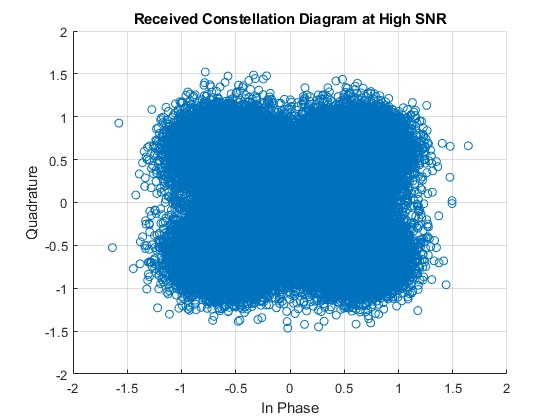
\includegraphics[width=0.8\linewidth]{OFDM Constellation Diagram}}
    		\caption{OFDM Constellation Diagram  (Rayleigh)}
  	  \end{figure}

The plot below represents the Bit Error Rate (BER) vs. Signal-to-Noise Ratio (SNR) performance of an OFDM system. It compares the measured BER from the simulation against the theoretical (reference) BER for the given modulation scheme and channel model. Both curves show a monotonic decrease in BER with increasing SNR, which is expected as higher SNR improves the signal quality and reduces errors. Around 6-10 dB, the curve begins to drop sharply, indicating the SNR threshold beyond which the system transitions from error-prone to error-free performance. This plot confirms that the OFDM system performs reliably under high SNR and aligns closely with theoretical predictions.
    
    \begin{figure}[H]
		\centering
    		\fbox{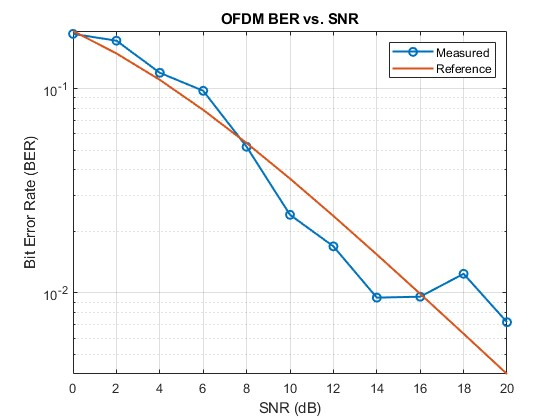
\includegraphics[width=0.8\linewidth]{OFDM BER vs SNR}}
    		\caption{OFDM BER vs. SNR}
  	  \end{figure}
    

    
    
    
    
    \section {JRC}

	Conflict

	\end{enumerate}
	
	
	\bibliographystyle {IEEEtran}
	\bibliography {References}
	
		
	
	
	%\nocite{yang_subcarrier_multiplexing}
	%\bibliography{sources}{}
   % \bibliographystyle{ieeetr}
  
\end{document}

%\begin{equation}
%y = x^2
%\end{equation}
%\Delta{R} = \frac{c}{2\Beta}